% !TEX program = xelatex
\documentclass[12pt,a4paper]{article}

\usepackage[UTF8,scheme=chinese]{ctex}
\usepackage{geometry}
\usepackage{graphicx}
\usepackage{booktabs}
\usepackage{longtable}
\usepackage{hyperref}
\usepackage{amsmath}
\usepackage{listings}
\usepackage{xcolor}
\usepackage{enumitem}
\usepackage{tikz}
\usetikzlibrary{arrows.meta,positioning,shapes.geometric}

\geometry{left=2.5cm,right=2.5cm,top=2.8cm,bottom=2.8cm}

\hypersetup{
    colorlinks=true,
    linkcolor=blue,
    urlcolor=blue,
    citecolor=blue
}

\lstset{
    basicstyle=\ttfamily\small,
    breaklines=true,
    frame=single,
    backgroundcolor=\color{gray!8},
    keywordstyle=\color{blue},
    commentstyle=\color{green!50!black},
    numbers=left,
    numberstyle=\tiny\color{gray},
    tabsize=4
}

\title{\textbf{MAVLink 协议调研与开发环境搭建报告} \\ \large 环境配置、SITL 仿真与 QGroundControl 连接验证}
\author{实习周报成果}
\date{2026年7月1日}

\begin{document}

\maketitle
\tableofcontents
\newpage

%==============================================================================
\section{MAVLink 协议调研}
%==============================================================================

\subsection{MAVLink 概述}

MAVLink（Micro Air Vehicle Link）是一种轻量级、开源的无人机通信协议，最初由苏黎世联邦理工学院（ETH Zurich）的 Lorenz Meier 等人于 2009 年前后提出，旨在为微型飞行器提供统一的机载消息格式与地面站交互能力。经过多年发展，MAVLink 已成为开源飞控生态（ArduPilot、PX4 等）与地面站（QGroundControl、Mission Planner 等）之间通信的事实标准。

\textbf{设计目标}主要包括：
\begin{itemize}[leftmargin=2em]
    \item \textbf{轻量}：单条消息头部仅 10 字节（MAVLink 2），适合带宽受限的无线链路；
    \item \textbf{开源}：消息定义以 XML 描述，可自动生成多语言编解码库；
    \item \textbf{通用}：覆盖心跳、姿态、GPS、任务、参数、命令等数百种标准消息类型；
    \item \textbf{可扩展}：支持厂商自定义消息及 MAVLink 2 的签名认证机制。
\end{itemize}

当前行业地位：在开源无人机领域，MAVLink 2 几乎是飞控与地面站之间的默认应用层协议；商用领域亦广泛采用或兼容该协议栈。

\subsection{与其他通信方案的对比}

\begin{table}[htbp]
\centering
\caption{MAVLink 与 DDS、ROS 通信层对比}
\begin{tabular}{p{2.2cm}p{3.8cm}p{3.8cm}p{3.8cm}}
\toprule
\textbf{维度} & \textbf{MAVLink} & \textbf{DDS} & \textbf{ROS/ROS2 通信} \\
\midrule
定位 & 无人机专用应用层消息协议 & 通用分布式中间件 & 机器人框架内置通信层 \\
消息模型 & 预定义二进制消息 ID + 载荷 & Topic/Service，IDL 定义 & Topic/Service/Action \\
典型链路 & 串口、UDP、TCP & 以太网、共享内存等 & 共享内存、UDP、DDS（ROS2） \\
资源占用 & 极低，适合嵌入式 & 相对较高 & 中等，依赖节点图 \\
适用场景 & 机载飞控 $\leftrightarrow$ 地面站/ companion & 多节点分布式系统、自动驾驶 & 机载计算、仿真、算法验证 \\
\bottomrule
\end{tabular}
\end{table}

\textbf{小结}：MAVLink 面向“飞控—地面站”这一垂直场景做了高度优化；DDS 更适合复杂分布式系统；ROS 通信层更适合机载算法与仿真生态。本实习以 MAVLink 为主线，因其与 QGC、ArduPilot SITL 的直接兼容性最好。

\subsection{系统架构与角色划分}

\begin{figure}[htbp]
\centering
\begin{tikzpicture}[
    node distance=1.2cm and 1.8cm,
    box/.style={draw, rounded corners, minimum width=2.6cm, minimum height=0.9cm, align=center, font=\small},
    proto/.style={draw, dashed, rounded corners, minimum width=2.2cm, minimum height=0.8cm, align=center, font=\small}
]
    \node[box, fill=blue!12] (gcs) {地面站\\QGroundControl};
    \node[proto, right=of gcs, fill=yellow!15] (mav) {MAVLink 2\\应用层协议};
    \node[box, right=of mav, fill=green!12] (fc) {飞控\\ArduPilot};
    \node[box, below=1.4cm of mav, fill=gray!12] (link) {物理链路\\UDP / 串口 / Wi-Fi};
    \node[box, below=1.4cm of fc, fill=orange!12] (sitl) {SITL 仿真\\sim\_vehicle.py};

    \draw[-{Stealth}] (gcs) -- node[above,font=\scriptsize]{双向消息} (mav);
    \draw[-{Stealth}] (mav) -- (fc);
    \draw[-{Stealth}] (mav) -- (link);
    \draw[-{Stealth}] (link) -- (sitl);
    \draw[-{Stealth},dashed] (fc) -- (sitl);
\end{tikzpicture}
\caption{地面站—协议—飞控（SITL）关系示意}
\label{fig:arch}
\end{figure}

各组件角色如下：
\begin{itemize}[leftmargin=2em]
    \item \textbf{QGroundControl（QGC）}：地面控制站，负责任务规划、参数配置、飞行监控及 MAVLink 消息可视化；
    \item \textbf{ArduPilot}：开源飞控固件；在 SITL 模式下于主机/虚拟机中模拟真实飞控行为；
    \item \textbf{MAVLink}：定义消息格式与语义，与底层传输无关；
    \item \textbf{物理链路}：本实验采用 UDP（默认端口 14550）；实际飞行可使用数传电台、Wi-Fi、4G 等；
    \item \textbf{Python / pymavlink}：用于脚本级 MAVLink 交互，适合自动化测试与二次开发。
\end{itemize}

\subsection{技术选型分析}

\subsubsection{MAVLink 与物理层的适配}

MAVLink 作为应用层协议，通过 \texttt{mavlink\_connection} 等接口适配多种传输方式：
\begin{itemize}[leftmargin=2em]
    \item \textbf{串口（Serial）}：典型用于飞控直连或数传电台，波特率常见 57600/115200；
    \item \textbf{UDP}：SITL 仿真与地面站本地通信的首选，延迟低、配置简单；
    \item \textbf{TCP}：适用于可靠连接场景，SITL 内部亦使用 TCP 5760 连接仿真核心与 MAVProxy。
\end{itemize}

\subsubsection{选型理由：Python + ArduPilot SITL + QGC}

\begin{table}[htbp]
\centering
\caption{本实验技术栈选型理由}
\begin{tabular}{p{3.5cm}p{9.5cm}}
\toprule
\textbf{组件} & \textbf{选型理由} \\
\midrule
Python + pymavlink & 语法简洁、库成熟、便于快速验证消息收发与后续脚本开发 \\
ArduPilot SITL & 无需真实飞机即可复现完整飞控逻辑，与 QGC 生态无缝衔接 \\
QGroundControl & 开源、支持 MAVLink 2、内置 MAVLink Inspector，便于教学与调试 \\
Ubuntu 虚拟机 & ArduPilot 官方工具链面向 Linux，在 Windows 宿主上通过 VM 运行 SITL 是常见方案 \\
\bottomrule
\end{tabular}
\end{table}

%==============================================================================
\section{开发环境配置文档}
%==============================================================================

\subsection{总体环境说明}

\begin{table}[htbp]
\centering
\caption{软硬件环境一览}
\begin{tabular}{ll}
\toprule
\textbf{项目} & \textbf{配置} \\
\midrule
宿主操作系统 & Windows 10（版本 10.0.22000） \\
虚拟机 & VMware Workstation + Ubuntu（桌面版） \\
宿主 Python & Python 3.10.7 \\
地面站 & QGroundControl 4.2（支持 MAVLink 2） \\
飞控仿真 & ArduPilot SITL（ArduCopter，Copter-4.4 分支） \\
Windows 编译工具链（可选） & Visual Studio Build Tools（MSVC v14.29），路径 \texttt{D:\textbackslash Microsoft Visual Studio} \\
Qt 环境（可选，源码编译 QGC 用） & Qt 5.15.2 MSVC2019 64-bit，Qt Creator，CMake 3.29.3，路径 \texttt{D:\textbackslash Qt6} \\
版本管理 & Git 2.47.0 \\
\bottomrule
\end{tabular}
\end{table}

本报告实验路径采用\textbf{Windows 宿主运行 QGC + Ubuntu 虚拟机运行 ArduPilot SITL} 的分离架构；Qt/MSVC 环境作为从源码构建 QGC 的预备能力一并记录。

\subsection{Windows 侧环境配置流程}

\subsubsection{安装 Git 并修复 SSL 问题}

安装 Git for Windows 后，克隆 GitHub 仓库时出现：
\begin{lstlisting}[language=bash]
fatal: unable to access 'https://github.com/...':
SSL certificate problem: unable to get local issuer certificate
\end{lstlisting}

\textbf{解决方案}：将 Git SSL 后端切换为 Windows 原生证书库：
\begin{lstlisting}[language=bash]
git config --global http.sslBackend schannel
\end{lstlisting}

\subsubsection{安装 QGroundControl}

从 QGC 4.2 发布页下载 \texttt{QGroundControl-installer.exe} 并安装。QGC 4.2 默认支持 MAVLink 2，无需额外配置协议版本。

\subsubsection{安装 Visual Studio Build Tools（MSVC）}

为后续可选的 QGC 源码编译，安装 Visual Studio Build Tools，勾选“使用 C++ 的桌面开发”，包含 MSVC v142 与 Windows 10/11 SDK。实际安装路径为 \texttt{D:\textbackslash Microsoft Visual Studio}（非默认 C 盘路径），导致初期检测脚本未识别，需手动在 Qt Creator 中配置编译器。

\subsubsection{安装与配置 Qt 5.15.2}

通过 Qt 维护工具（MaintenanceTool）在已有 Qt 6.8.0 环境中\textbf{追加安装} Qt 5.15.2 MSVC2019 64-bit，路径为 \texttt{D:\textbackslash Qt6\textbackslash 5.15.2\textbackslash msvc2019\_64}。

\textbf{Qt Creator Kit 配置难点}：
\begin{enumerate}[leftmargin=2em]
    \item 新建 Kit 后 Compiler 显示 \texttt{<No compiler>}，需手动添加 MSVC；
    \item Initialization 须指向 \texttt{vcvarsall.bat} 并选择参数 \texttt{amd64}，不可使用 \texttt{x86}；
    \item ABI 须为 \texttt{x86-windows-msvc2019-pe-64bit}，与 Qt 5.15.2 MSVC2019 套件匹配；
    \item C 与 C++ 编译器需分别添加并绑定到 Kit。
\end{enumerate}

\subsection{Ubuntu 虚拟机侧：ArduPilot SITL 配置}

\subsubsection{创建虚拟机并安装 Ubuntu}

在 VMware 中创建 Ubuntu 虚拟机，分配不少于 4\,GB 内存与 40\,GB 磁盘。ArduPilot 官方工具链主要面向 Linux，故 SITL 运行于虚拟机内。

\subsubsection{克隆 ArduPilot 源码}

\begin{lstlisting}[language=bash]
cd ~
git clone https://github.com/ArduPilot/ardupilot.git
cd ardupilot
git checkout Copter-4.4
git submodule update --init --recursive
\end{lstlisting}

源码存放于 \texttt{\~/桌面/ArduPilot/ardupilot}。必须使用 \texttt{--recursive} 或 \texttt{submodule update}，否则依赖库缺失将导致编译失败。

\subsubsection{安装 Python 与系统依赖}

\begin{lstlisting}[language=bash]
cd ~/ardupilot
Tools/environment_install/install-prereqs-ubuntu.sh -y
\end{lstlisting}

安装完成后需\textbf{关闭并重新打开终端}，使命令行环境变量生效。此后可直接使用 \texttt{sim\_vehicle.py}，或显式调用：
\begin{lstlisting}[language=bash]
python3 ../Tools/autotest/sim_vehicle.py -v ArduCopter --console --map
\end{lstlisting}

\subsubsection{首次启动 SITL}

首次运行会自动编译 ArduCopter SITL 目标，耗时约 2--30 分钟。成功标志包括：
\begin{itemize}[leftmargin=2em]
    \item \texttt{build finished successfully}
    \item \texttt{Detected vehicle 1:1 on link 0}
    \item \texttt{Received 1339 parameters}
    \item 控制台提示符为 \texttt{STABILIZE>}
\end{itemize}

\subsection{环境配置中的主要难点与解决方案}

\begin{longtable}{p{3.2cm}p{4.5cm}p{5.8cm}}
\toprule
\textbf{问题现象} & \textbf{原因分析} & \textbf{解决方法} \\
\midrule
\endhead
Git 克隆 SSL 失败 & OpenSSL 证书链与系统不一致 & \texttt{git config --global http.sslBackend schannel} \\
\midrule
Qt 在线安装器验证失败 & 账号/网络无法访问 Qt 服务器 & 使用离线安装包或国内镜像；网页重置密码后重试 \\
\midrule
Qt Kit 黄色警告 & MSVC 未绑定或 ABI/架构错误 & 手动添加 \texttt{vcvarsall.bat + amd64}，绑定 Qt 5.15.2 \\
\midrule
\texttt{sim\_vehicle.py: 未找到命令} & 未执行 install-prereqs 或 PATH 未生效 & 运行官方安装脚本并重启终端 \\
\midrule
\texttt{UDP ports must be specified as host:port} & \texttt{--out} 参数缺少端口号 & 使用 \texttt{--out=udp:IP:14550} 格式 \\
\midrule
使用公网 IP（如 26.x.x.x）无法连接 & 虚拟机路由不可达该地址 & 改用桥接模式 + Windows 局域网 IP \\
\midrule
ping 宿主机失败 & 虚拟机为 NAT 模式 & 改为桥接模式并重启虚拟机 \\
\midrule
SITL 正常但 QGC 仍 Disconnected & MAVLink 未发往 Windows；或端口冲突 & 添加 \texttt{--out=udp:WindowsIP:14550}；关闭 QGC 中 NMEA 对 14550 端口的占用；放行防火墙 UDP 14550 \\
\bottomrule
\caption{环境搭建主要问题与解决方案}
\end{longtable}

%==============================================================================
\section{连接与验证}
%==============================================================================

\subsection{网络连接配置}

最终将 VMware 网络适配器设置为\textbf{桥接模式}，使 Ubuntu 虚拟机与 Windows 宿主处于同一局域网。在 Windows 上通过 \texttt{ipconfig} 获取 IPv4 地址（形如 \texttt{192.168.x.x}），在虚拟机中启动 SITL 时显式指定 MAVLink 输出：

\begin{lstlisting}[language=bash]
cd ~/桌面/ArduPilot/ardupilot/ArduCopter
python3 ../Tools/autotest/sim_vehicle.py -v ArduCopter --console --map \
    --out=udp:<Windows主机IP>:14550
\end{lstlisting}

QGC 侧在“应用设置”中启用 UDP 自动连接；需确保 NMEA GPS 流不使用 14550 端口，以免与 MAVLink 默认监听端口冲突。Windows 防火墙需允许入站 UDP 14550。

\subsection{QGC 连接 SITL 验证}

连接成功后，QGC 顶部状态由 \texttt{Disconnected} 变为 \texttt{Connected}，地图显示仿真飞机位置，遥测数据（高度、速度等）开始刷新。

\subsection{MAVLink Inspector 消息观察}

在 QGC 中选择 \textbf{Analyze $\rightarrow$ MAVLink Inspector}，对以下 MAVLink 2 消息进行观察与记录：

\begin{table}[htbp]
\centering
\caption{关键 MAVLink 2 消息说明}
\begin{tabular}{p{3.2cm}p{9.8cm}}
\toprule
\textbf{消息名称} & \textbf{观察要点} \\
\midrule
HEARTBEAT & 心跳包，约 1\,Hz 周期刷新；含飞行器类型、飞行模式、系统状态 \\
GPS\_RAW\_INT & 原始 GNSS 数据：纬度、经度、高度及定位精度相关字段 \\
SYS\_STATUS & 系统状态：传感器健康、电池电压、负载等 \\
COMMAND\_LONG & 地面站下发的长命令（解锁、起飞、模式切换等） \\
\bottomrule
\end{tabular}
\end{table}

\subsection{操作与指令消息联动验证}

在 QGC 飞行界面依次执行解锁、起飞与飞行模式切换操作，并在 MAVLink Inspector 中同步观察对应消息。需要说明的是，Inspector 默认主要展示从飞控接收的消息；地面站下发的 \texttt{COMMAND\_LONG} 不一定出现在列表中，但飞控返回的 \texttt{COMMAND\_ACK}（命令确认）可在操作瞬间观察到，同样能够证明指令已成功下发并被飞控接受。

\begin{enumerate}[leftmargin=2em]
    \item \textbf{解锁（Arm）}：Inspector 中出现 \texttt{COMMAND\_ACK}，\texttt{command} 字段对应解锁相关命令，\texttt{result}=0 表示命令被接受；
    \item \textbf{起飞（Takeoff）}：同样可观察到 \texttt{COMMAND\_ACK} 消息刷新；
    \item \textbf{切换飞行模式}：\texttt{COMMAND\_ACK} 中 \texttt{command}=176（\texttt{MAV\_CMD\_DO\_SET\_MODE}），\texttt{result}=0 表示模式切换成功。
\end{enumerate}

上述操作与消息观察均已完成，证明地面站、MAVLink 协议栈与 SITL 仿真飞控之间通信正常。验证截图见下文图~\ref{fig:qgc-connected}--图~\ref{fig:command-ack-mode}。

\subsection{验证截图}

\begin{figure}[htbp]
\centering
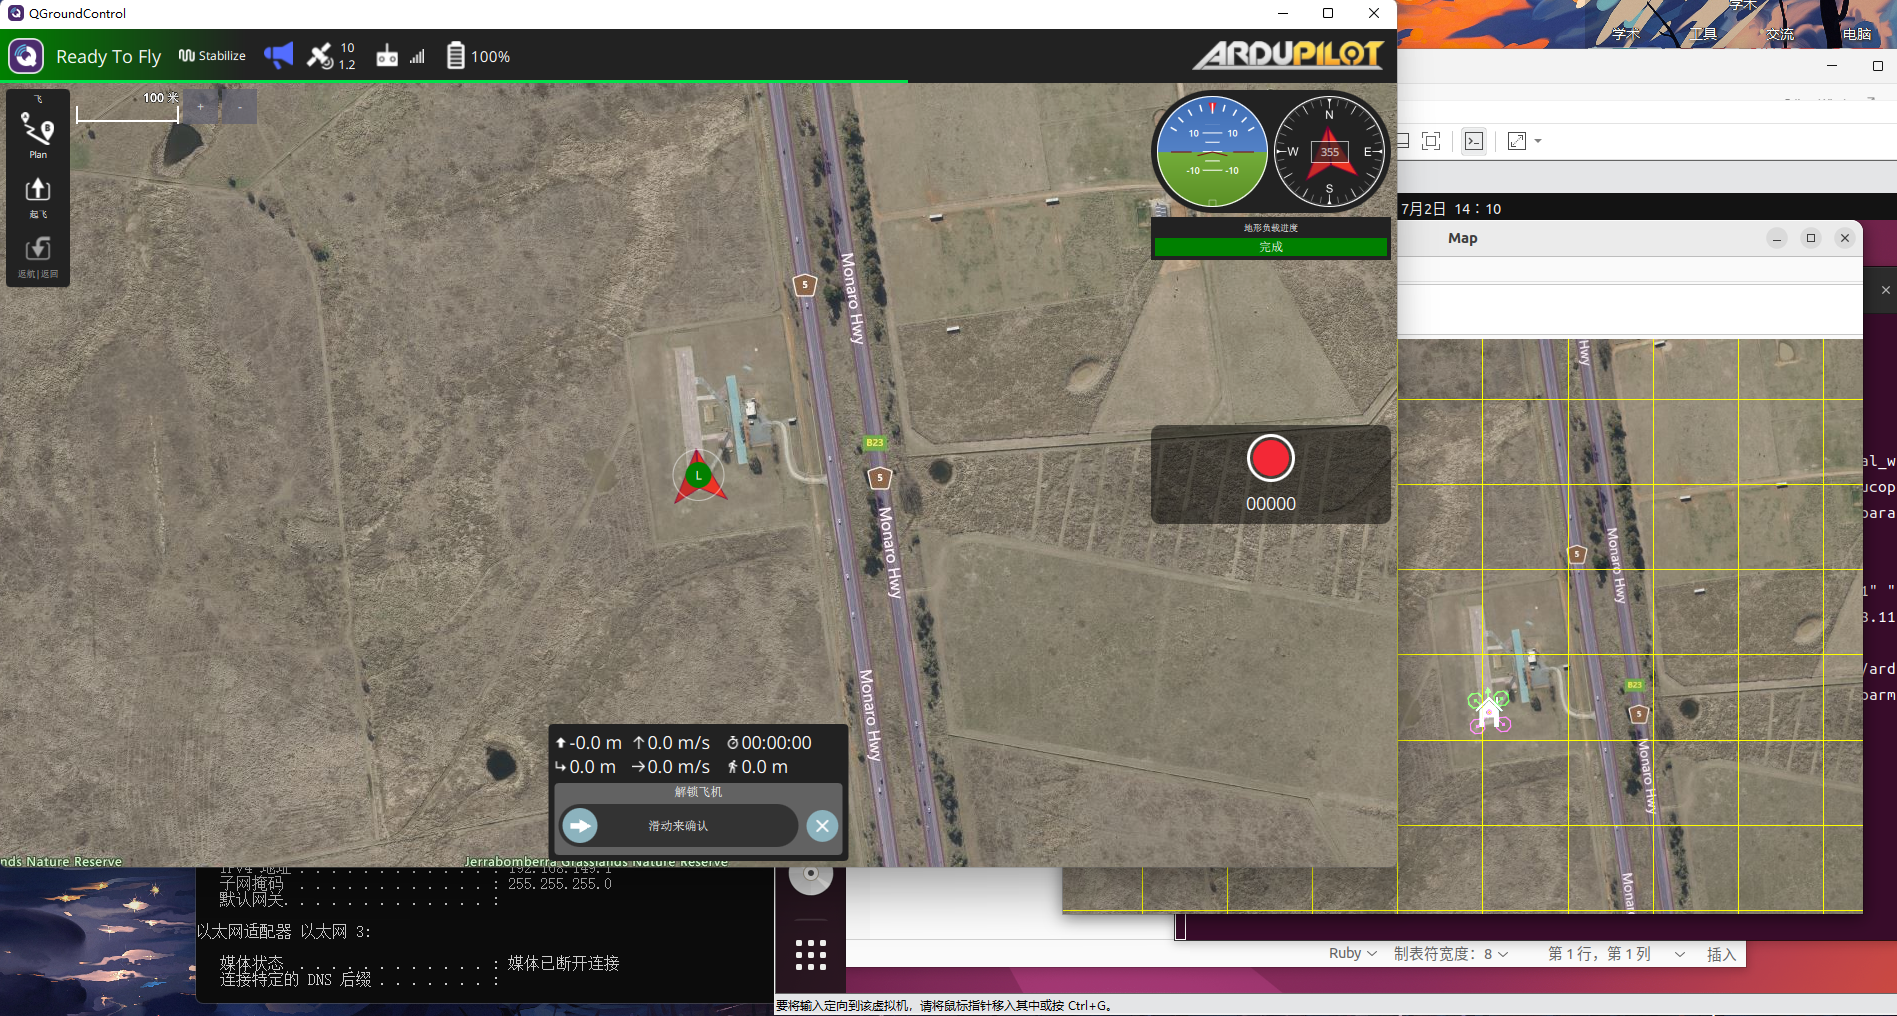
\includegraphics[width=0.92\textwidth]{screenshots/qgc_connected.png}
\caption{QGC 与 SITL 连接成功界面}
\label{fig:qgc-connected}
\end{figure}

\begin{figure}[htbp]
\centering
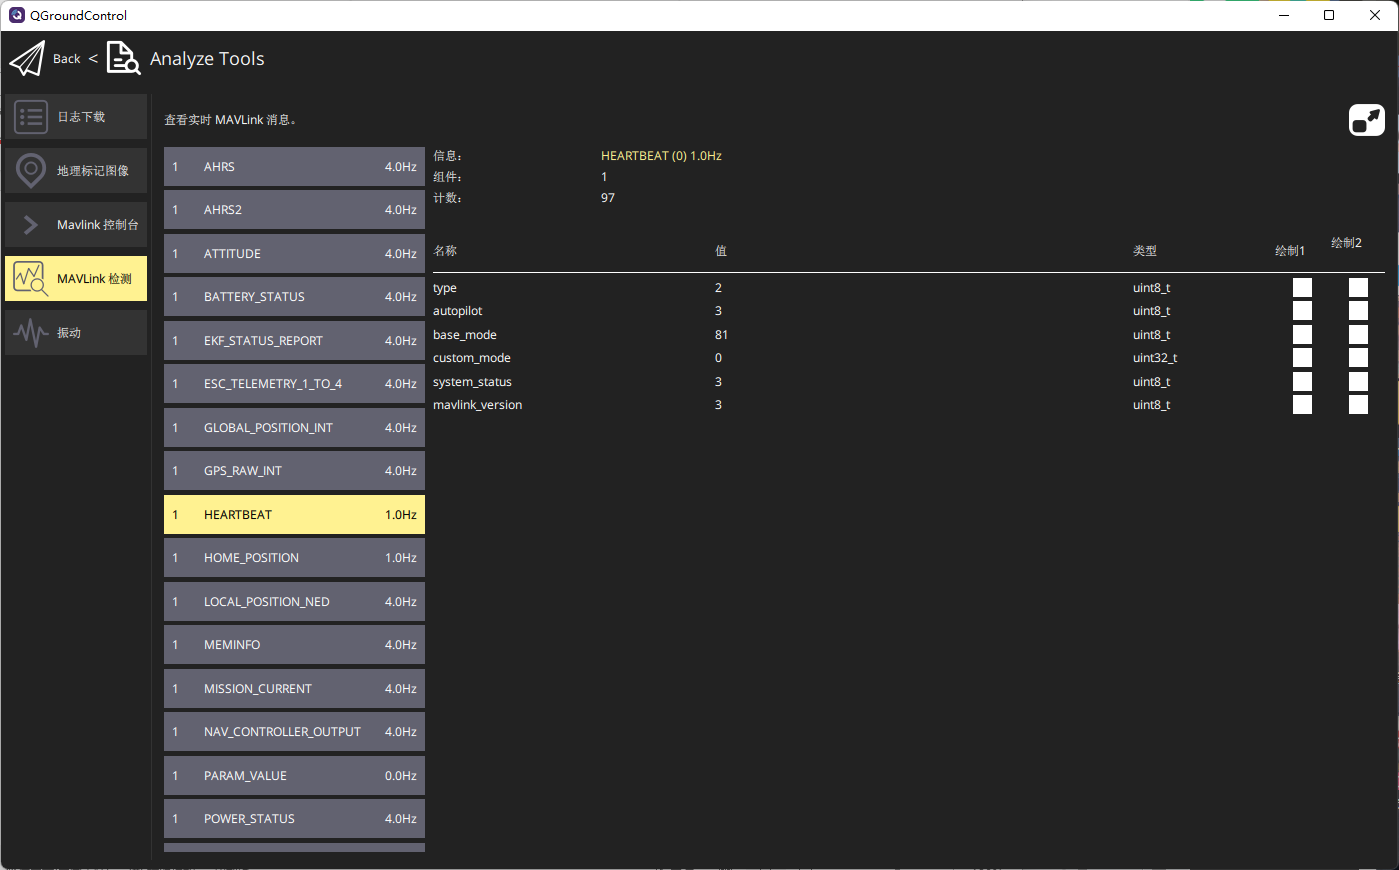
\includegraphics[width=0.92\textwidth]{screenshots/mavlink_inspector_messages.png}
\caption{MAVLink Inspector 关键消息观察（HEARTBEAT、GPS\_RAW\_INT、SYS\_STATUS 等）}
\label{fig:mavlink-messages}
\end{figure}

\begin{figure}[htbp]
\centering
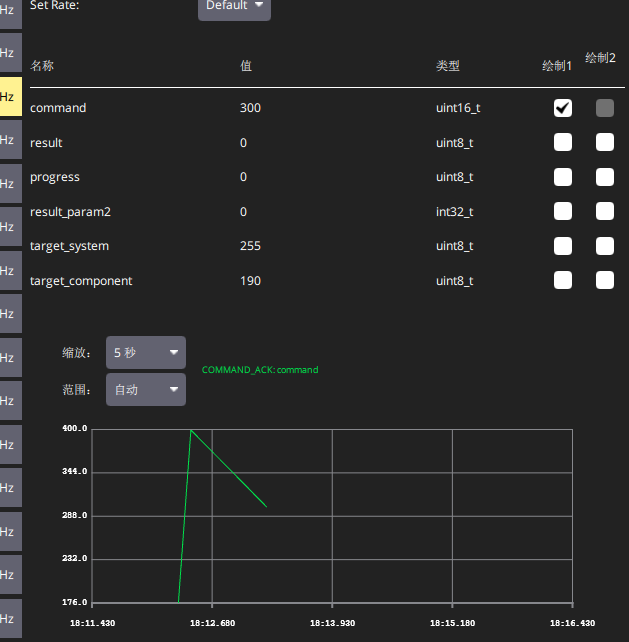
\includegraphics[width=0.75\textwidth]{screenshots/command_ack_arm.png}
\caption{解锁/起飞操作触发的 COMMAND\_ACK 消息（command 字段变化，result=0 表示命令被接受）}
\label{fig:command-ack-arm}
\end{figure}

\begin{figure}[htbp]
\centering
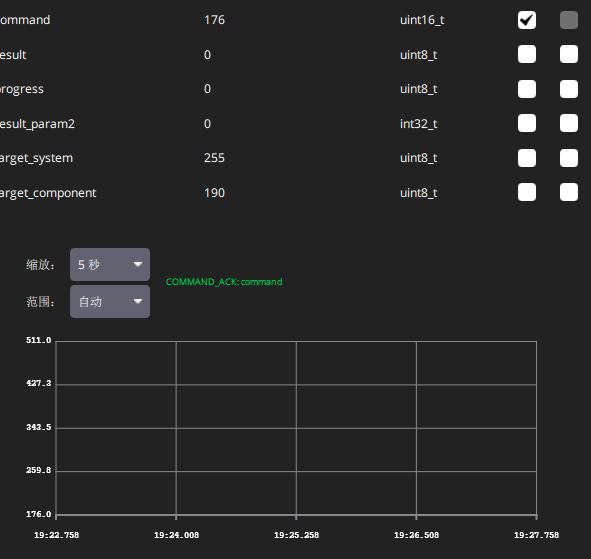
\includegraphics[width=0.75\textwidth]{screenshots/command_ack_mode.png}
\caption{飞行模式切换时的 COMMAND\_ACK 消息（command=176，MAV\_CMD\_DO\_SET\_MODE）}
\label{fig:command-ack-mode}
\end{figure}

%==============================================================================
\section{总结与后续工作}
%==============================================================================

本周完成了 MAVLink 协议调研、Windows/Linux 混合开发环境搭建、ArduPilot SITL 仿真启动以及 QGroundControl 与 SITL 的 MAVLink 2 连接验证。环境搭建过程中，Qt Kit 配置、虚拟机网络桥接与 MAVLink UDP 端口转发是主要难点，均已通过查阅文档与逐步排查解决。

\textbf{后续计划}（对应实习任务安排）：
\begin{itemize}[leftmargin=2em]
    \item 使用 Python 与 pymavlink 编写 \texttt{basic\_communication.py} 等基础交互脚本；
    \item 实现参数读写、任务上传、命令控制等高级功能；
    \item 启用并验证 MAVLink 2 安全签名；
    \item 完成地理围栏监测与自动悬停/返航脚本开发。
\end{itemize}

\end{document}
